\documentclass[10pt,twocolumn]{article}

\usepackage[T1]{fontenc}
\usepackage[utf8]{inputenc}
\usepackage{lmodern}
\usepackage{microtype}
\usepackage{amsmath,amssymb}
\usepackage{booktabs,array}
\usepackage{tikz}
\usepackage{url}
\usepackage[hidelinks]{hyperref}
\usetikzlibrary{arrows.meta,positioning,shapes.geometric}

\setlength{\textfloatsep}{8pt plus 1pt minus 2pt}
\setlength{\floatsep}{8pt plus 1pt minus 2pt}
\setlength{\intextsep}{8pt plus 1pt minus 2pt}
\setlength{\parskip}{2pt}
\setlength{\parindent}{1em}
\sloppy

\title{SessionBound: Turning Enterprise Task Approval into Budgeted Database Sessions}
\author{Minmin Wu\\Independent Researcher}
\date{}
\hypersetup{
  pdftitle={SessionBound: Turning Enterprise Task Approval into Budgeted Database Sessions},
  pdfauthor={Minmin Wu}
}

\begin{document}

\twocolumn[
\begin{@twocolumnfalse}
\maketitle
\begin{abstract}
Enterprise AI agents are useful for internal analysis, audit, compliance
review, and operational investigation, but they create a difficult
authorization problem. A manager or data owner may approve a business
task, while the agent later generates open-ended SQL below the
application layer. Existing systems help identify agents, delegate
authority, govern data products, or enforce database policy, but they do
not directly turn an approved enterprise task into a bounded database
execution context. SessionBound fills this gap. It turns approved
enterprise tasks into short-lived, budgeted, and auditable database
sessions for AI agents. A control plane defines task templates, accepts
task applications, records approvals, assigns budgets, and issues signed
task tokens. A database runtime, SessionBoundDB, binds a token to a
session and enforces safe views, row scope, denied fields, operation
limits, query budgets, disclosure budgets, and receipts. The database
does not rely on an LLM to decide whether a query is safe. The agent may
generate SQL freely, but each attempt must stay inside the approved
boundary. A PostgreSQL prototype passed a 24-scenario validation suite.
Microbenchmarks show p50 SessionBound execution around 1.4--1.5 ms
versus raw PostgreSQL p50 around 0.052--0.074 ms on small synthetic
queries: high relative overhead, but low absolute latency.
\end{abstract}
\vspace{0.5em}
\end{@twocolumnfalse}
]

\section{Introduction}

AI agents change how enterprise users interact with data. A user no
longer needs to know which report exists, which dashboard to open, or
which endpoint exposes a particular slice of operational data. The user
can ask an agent to inspect travel reimbursements for one department,
find unusual merchants, compare monthly totals, and drill into claims
near approval thresholds. These tasks are temporary, exploratory,
cross-table, and often under-specified. They are also the tasks for
which a fixed SaaS screen is least likely to exist.

The security problem is that exploratory SQL cannot simply be trusted to
the agent. Giving an agent raw database access is unsafe. Prompting the
agent not to inspect salary, bank, or unrelated department data is not a
security boundary. Requiring a business approver to write row-level
database policy for every temporary analysis is unrealistic. In real
enterprises, people approve tasks, scopes, and budgets above the
database. The database still needs a precise execution boundary below
the application layer.

SessionBound is based on a simple principle: business users approve
tasks, not database policies. Agents generate SQL, but databases enforce
the approved boundary. A business approval becomes a signed task token.
The token binds an agent, credential, task scope, safe views, denied
fields, lifetime, operation limits, query budget, disclosure budget, and
policy version. The database runtime consumes that token and creates a
budgeted database session. The agent remains free to generate useful
SQL, but every query attempt is checked deterministically.

This paper presents a shortened version of the SessionBound design. It
makes three contributions. First, it identifies enterprise task approval
as the missing layer between agent delegation and database enforcement.
Second, it proposes a control-plane and runtime architecture for
turning approvals into budgeted database sessions. Third, it reports a
PostgreSQL prototype that validates core enforcement behavior and
measures small-query overhead.

\section{Motivation and Threat Model}

Enterprise analytical work often starts with approval rather than
database policy. A manager may approve a monthly expense review for the
Sales department in June 2026. A data owner may allow employee names and
reimbursement amounts, but not salaries, bank accounts, phone numbers,
or other departments. A compliance reviewer may require a short
expiration time, a maximum number of queries, and an audit trail. These
decisions are natural business decisions. They are not naturally written
as SQL predicates by the approver.

The agent, however, operates at the SQL layer. It may join safe business
objects, rank rows, aggregate by department, inspect outliers, and
generate follow-up queries. This open-endedness is the value of the
agent. It is also the risk. If the system only authorizes a tool call,
the generated query may still attempt raw-table access, denied columns,
DDL, mutations, catalog inspection, broad joins, repeated probing, or
payload aggregation that hides many records inside one result cell.

SessionBound assumes the following threat model. The agent may be
curious, faulty, prompt-injected, or directly instructed to exceed the
approved boundary. It may generate arbitrary SQL strings. It may try to
read raw tables, denied fields, out-of-scope rows, system catalogs, or
large payloads. It may repeat queries until a budget is exhausted. The
agent is not trusted to interpret the task correctly, and an LLM is not
trusted as the runtime security oracle.

SessionBound does not assume a malicious database administrator, a
compromised signing key, or a database engine whose access-control
mechanisms have been bypassed. It also does not claim to eliminate all
semantic inference. If allowed query answers reveal correlated
information, an agent may infer facts that were not directly exposed.
Disclosure budgets account for and limit exposure during one task
session; they are not differential privacy~\cite{dwork2014algorithmic}.

The intended protection target is the direct boundary between approved
task authority and database execution. SessionBound should deny direct
access to unauthorized schemas and fields, enforce row scope, reject
unsupported operations, stop sessions after expiration or revocation,
track cumulative exposure, and emit receipts for both allowed and
denied attempts.

\section{SessionBound Design}

SessionBound separates three concerns. The control plane records what
the organization approved. The agent execution layer decides which SQL
queries to try. The database runtime enforces how the approved authority
may be spent. Figure~\ref{fig:architecture} shows the architecture.

\begin{figure*}[t]
\centering
\resizebox{0.92\textwidth}{!}{%
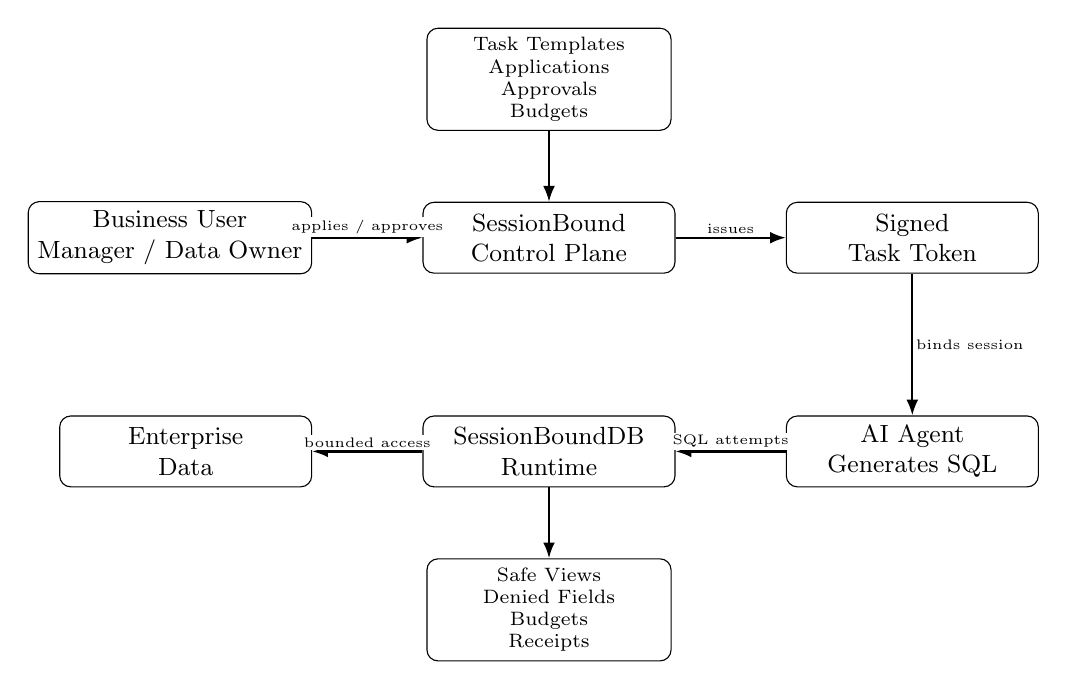
\begin{tikzpicture}[
  node distance=9mm and 14mm,
  box/.style={draw, rounded corners, align=center, minimum width=32mm, minimum height=9mm, font=\small},
  smallbox/.style={draw, rounded corners, align=center, minimum width=31mm, minimum height=8mm, font=\scriptsize},
  arrow/.style={-{Latex[length=2mm]}, thick},
  edgelabel/.style={font=\tiny, fill=white, inner sep=1pt}
]
\node[box] (business) {Business User\\Manager / Data Owner};
\node[box, right=of business] (control) {SessionBound\\Control Plane};
\node[box, right=of control] (token) {Signed\\Task Token};
\node[smallbox, above=of control] (template) {Task Templates\\Applications\\Approvals\\Budgets};
\node[box, below=18mm of control] (runtime) {SessionBoundDB\\Runtime};
\node[box, left=of runtime] (data) {Enterprise\\Data};
\node[box, right=of runtime] (agent) {AI Agent\\Generates SQL};
\node[smallbox, below=of runtime] (enforce) {Safe Views\\Denied Fields\\Budgets\\Receipts};
\draw[arrow] (business) -- node[above, edgelabel]{applies / approves} (control);
\draw[arrow] (control) -- node[above, edgelabel]{issues} (token);
\draw[arrow] (token) -- node[right, edgelabel]{binds session} (agent);
\draw[arrow] (agent) -- node[above, edgelabel]{SQL attempts} (runtime);
\draw[arrow] (runtime) -- node[above, edgelabel]{bounded access} (data);
\draw[arrow] (template) -- (control);
\draw[arrow] (runtime) -- (enforce);
\end{tikzpicture}
}
\caption{SessionBound architecture. The control plane turns enterprise task approval into a signed task token; the agent may generate SQL freely, but SessionBoundDB enforces safe views, denied fields, budgets, and receipts inside the database session.}
\label{fig:architecture}
\end{figure*}

\subsection{Control Plane}

A task template describes a reusable class of work that may be delegated
to an agent once scoped and approved. For example, a monthly expense
anomaly review template might allow safe views for expenses, employees,
and departments; deny salary, bank-account, and phone fields; require
tenant, month, and department scope; allow only read operations; and set
default query and disclosure budgets. The template is created by a data
platform or application team, not by the agent.

A task application instantiates a template with a concrete requester,
actor, scope, and reason. An approval decides whether that scoped task
should exist. Approval may be automatic, role-based, or manual. The
important property is that the approver decides on a business task, not
on a hand-written database policy.

After approval, the control plane issues a signed task token. A task
token contains fields such as \texttt{task\_id}, actor,
\texttt{credential\_id}, allowed safe views, denied fields, row scope,
TTL, query budget, disclosure budget, safe-view registry version,
policy version, audience, nonce, and signature. The token is a compact
authorization object that the database runtime can validate without
asking an LLM to interpret the natural-language task.

\subsection{Safe Views and Scope}

SessionBound exposes data through registered safe views rather than raw
tables. A safe view is a governed business object with an explicit
column list, row-scope binding, and registry version. Safe views should
avoid \texttt{SELECT *}; adding a new exposed column changes the
exposure boundary and should invalidate incompatible task tokens. This
keeps schema drift from silently broadening existing approvals.

Row scope is bound to the task token. A query for another month or
department should not reveal data merely because the agent wrote a
broader predicate. In the prototype, out-of-scope access through safe
views is transparently filtered to zero rows rather than treated as an
explicit denial. Raw-table access, denied-field access, catalog escape,
mutations, and DDL are denied.

\subsection{Budgets and Receipts}

SessionBound treats budgets as authority accounting. Query budgets limit
the number of SQL attempts. Disclosure budgets limit the amount of
task-authorized information exposed during one session, for example by
result rows, bytes, or unique entity identifiers. A production budget
vector can assign different weights to detail rows, aggregate rows, and
high-sensitivity columns.

Receipts record how approved authority was spent. An allow receipt
records the task, credential, query identity, safe views touched, rows
returned, budget consumed, policy versions, and timestamp. A denial
receipt records the denied attempt and reason, such as denied column,
raw schema, unsupported operation, expired token, or budget exhaustion.
Receipts make the session auditable after the agent has completed its
work.

\section{Runtime Enforcement}

SessionBoundDB is the PostgreSQL-based reference runtime. The prototype
keeps the SQL schema name \texttt{taskbound} for compatibility with the
existing implementation, but the public project name is SessionBound.

The runtime binds one signed task token to one active database session.
Rebinding is denied. The token must be valid, unexpired, intended for
the database audience, and bound to the credential used by the session.
Credential-token binding prevents an agent from presenting a token with
one identity while executing through another.

At query time, the runtime applies a deterministic decision procedure:
verify an active binding; validate token freshness and revocation
state; parse or conservatively inspect the SQL attempt; restrict access
to allowed safe views; reject denied fields and blocked schemas; enforce
row scope; reject disallowed operation types; check remaining query and
disclosure budget; execute the query only if every check passes; and
emit an allow or denial receipt.

The prototype uses conservative SQL checks plus PostgreSQL security
boundaries. This is sufficient for the validation suite, but it is not a
claim of production-grade SQL parsing. A hardened implementation should
use database parser hooks, executor-level checks, or a complete AST
validation path. Conservative blocking is acceptable for a prototype
because false positives are safer than silent overexposure. For example,
the v1 prototype denies payload aggregation functions such as
\texttt{json\_agg}, \texttt{array\_agg}, \texttt{string\_agg},
\texttt{xmlagg}, and \texttt{row\_to\_json} unless a future template
explicitly permits them with strict byte-level budgets. Ordinary
analytical aggregates such as \texttt{count}, \texttt{sum},
\texttt{avg}, \texttt{min}, and \texttt{max} remain allowed.

The runtime is intentionally LLM-independent. It does not ask whether
the generated SQL is consistent with the user's prose. It checks whether
the SQL stays inside a structured boundary approved by the enterprise.
This distinction is important: SessionBound does not solve all
semantic-policy questions, but it makes the executable boundary
deterministic, signed, budgeted, and auditable.

\section{Evaluation}

The evaluation asks two questions. First, can the PostgreSQL prototype
enforce the intended direct boundaries for representative analytical and
adversarial SQL patterns? Second, what is the small-query overhead of
the SessionBound runtime path relative to raw PostgreSQL?

\subsection{Functional Validation}

The canonical validation suite passed 24 of 24 scenarios. Table
\ref{tab:validation} compresses the suite into major categories. The
allowed cases cover safe-view reads, joins, common table expressions,
grouped aggregation, window functions, and scoped drill-down. The denied
cases cover salary and bank-account fields, raw tables, mutation SQL,
DDL, system catalog access, payload aggregation, and exhausted budgets.
Out-of-scope month and department cases are enforced by transparent
scope filtering.

\begin{table}[t]
\centering
\small
\caption{Functional validation summary. The canonical suite passed 24 of 24 scenarios.}
\label{tab:validation}
\begin{tabular}{@{}p{0.38\columnwidth}p{0.17\columnwidth}p{0.29\columnwidth}@{}}
\toprule
Category & Cases & Observed result \\
\midrule
Allowed analysis over safe views & 6 & Allowed \\
Denied sensitive fields & 2 & Denied \\
Denied schema or catalog escape & 2 & Denied \\
Denied mutation or DDL & 2 & Denied \\
Denied payload aggregation & 8 & Denied \\
Out-of-scope rows & 2 & Scope-filtered \\
Budget exhaustion & 2 & Denied \\
\midrule
Total & 24 & Passed \\
\bottomrule
\end{tabular}
\end{table}

These results validate the intended direct enforcement boundary. They
do not prove that every SQL dialect feature is safely handled, nor do
they eliminate inference from allowed answers. They show that the
prototype can bind a task token to a PostgreSQL session and consistently
apply the core controls required by the design.

\subsection{Performance Microbenchmark}

The microbenchmark compared equivalent raw PostgreSQL queries against
the SessionBound path for five query patterns: simple \texttt{SELECT},
safe-view \texttt{JOIN}, \texttt{GROUP BY}, CTE, and window function.
Each pattern used 10 warmup iterations and 100 measured iterations. The
baseline used an admin/test role over raw application tables with
tenant and month predicates matching the task scope. The SessionBound
path bound a signed task token and executed through
\texttt{taskbound.run(sql)}. HTTP latency and dynamic credential
creation were excluded so the benchmark focused on database runtime
overhead.

\begin{table}[t]
\centering
\small
\caption{Performance microbenchmark comparing raw PostgreSQL and SessionBoundDB runtime execution. SB denotes SessionBound.}
\label{tab:performance}
\begin{tabular}{@{}lrrrr@{}}
\toprule
Pattern & Raw p50 & SB p50 & Overhead & Rows \\
\midrule
SELECT & 0.063 ms & 1.434 ms & 2168.4\% & 3 \\
JOIN & 0.060 ms & 1.503 ms & 2408.0\% & 3 \\
GROUP BY & 0.066 ms & 1.450 ms & 2088.7\% & 3 \\
CTE & 0.052 ms & 1.457 ms & 2702.8\% & 1 \\
Window & 0.074 ms & 1.500 ms & 1937.5\% & 5 \\
\bottomrule
\end{tabular}
\end{table}

Table~\ref{tab:performance} shows high relative overhead because the
raw PostgreSQL baseline is extremely small. The absolute SessionBound
p50 latency remains around 1.4--1.5 ms for these small synthetic
queries. Likely sources include PL/pgSQL dispatch, SQL text checks,
task-session lookup, safe-view evaluation, budget updates, unique-row
exposure accounting, payload-aggregation checks, and receipt insertion.
These results should not be generalized to larger datasets without
additional experiments.

\section{Related Work}

SessionBound is intended to compose with, not replace, existing
authorization and data-governance systems. OAuth 2.0 provides delegated
API authorization~\cite{rfc6749}. Authenticated Delegation establishes
who may act for whom and how agent authority is delegated
verifiably~\cite{south2025authenticateddelegation}. PAuth checks
whether a service or tool operation is implied by a
task~\cite{sharma2026pauth}. Data Product MCP governs discovery and
access for enterprise data products over MCP
interfaces~\cite{tonnarelli2026dataproductmcp,mcp2025specification}.
Oracle Deep Data Security shows the importance of identity- and
context-aware database enforcement~\cite{oracle2026deepdatasecuritydocs,oracle2026deepdatasecuritybrief}.
Zanzibar provides consistent relationship-based authorization at
scale~\cite{pang2019zanzibar}. PostgreSQL row security is an important
database-native mechanism for row-level predicates~\cite{postgresql2026rowsecurity}.
Classical inference-control work studies leakage from database query
answers~\cite{adam1989securitycontrol}.

\begin{table*}[t]
\centering
\small
\caption{Related work boundary.}
\label{tab:related}
\begin{tabular}{@{}p{0.22\textwidth}p{0.34\textwidth}p{0.34\textwidth}@{}}
\toprule
System or area & Primary question & SessionBound distinction \\
\midrule
Authenticated Delegation & Who may act for whom? & Turns delegated task authority into a bounded database session. \\
PAuth & Is a tool operation implied by a task? & Enforces a structured SQL boundary instead of judging every query against prose. \\
Data Product MCP & How do agents access governed data products? & Makes the approved task session, not the data product, the runtime object. \\
Oracle DDS / database policy & How are identity and context enforced near data? & Adds templates, approvals, signed task tokens, budgets, and receipts around database enforcement. \\
Zanzibar & How are relationship permissions checked consistently? & Accounts for cumulative exposure during exploratory database analysis. \\
Inference control / DP & How is leakage from query answers limited? & Uses operational disclosure budgets, not formal differential privacy. \\
\bottomrule
\end{tabular}
\end{table*}

The closest related area is enterprise data-product governance, because
it shares the motivation that agents should not freely roam enterprise
data. SessionBound differs by treating the approved task and its
database session as the first-class object. A session may span multiple
safe views, consume cumulative budget, and produce receipts for every
attempt. This is the layer between business approval and database
execution.

\section{Limitations and Conclusion}

The current prototype has several limitations. It targets a single
PostgreSQL database. SQL checks are conservative and are not a
production AST enforcement mechanism. Disclosure budget is not
differential privacy. Semantic inference is reduced and accounted for,
not eliminated. Payload aggregation is conservatively blocked rather
than fully modeled. View drift invalidation is a design requirement. The
performance results are small synthetic microbenchmarks, not production
workload measurements.

Despite these limitations, SessionBound captures a useful systems
boundary for enterprise AI agents. Business users approve tasks, not
database policies. Agents generate SQL, but databases enforce the
approved boundary. The control plane turns a scoped approval into a
signed token; the database runtime turns that token into a short-lived,
budgeted, receipt-bearing session. This lets enterprises preserve the
flexibility of agent-generated analysis while moving the security
decision from prompts and application conventions into deterministic
database enforcement.

\bibliographystyle{unsrt}
\bibliography{references}

\end{document}
